\documentclass[conference]{IEEEtran}

% ---- Packages ----
\usepackage[utf8]{inputenc}
\usepackage{graphicx}
\usepackage{booktabs}
\usepackage{array}
\usepackage{hyperref}
\usepackage{xcolor}
\usepackage{tikz}
\usepackage{listings}
\usepackage{enumitem}
\usepackage{caption}
\usepackage{cite}
\usepackage{microtype}
\usetikzlibrary{shapes,arrows.meta,positioning}

% ---- Spacing ----
\setlength{\textfloatsep}{4pt plus 1pt minus 1pt}
\setlength{\floatsep}{4pt plus 1pt minus 1pt}
\setlength{\intextsep}{4pt plus 1pt minus 1pt}
\setlength{\abovecaptionskip}{3pt}
\setlength{\belowcaptionskip}{0pt}
\setlength{\columnsep}{16pt}
\setlist{nosep, leftmargin=12pt, topsep=1pt}
\captionsetup{font=small, skip=2pt}

% ---- Colors ----
\definecolor{isroblue}{RGB}{0, 51, 102}
\definecolor{codegreen}{RGB}{0,120,0}
\definecolor{codegray}{RGB}{100,100,100}
\hypersetup{colorlinks=true, linkcolor=isroblue, urlcolor=isroblue, citecolor=isroblue}

% ---- Code style ----
\lstset{
    basicstyle=\ttfamily\tiny,
    keywordstyle=\color{isroblue}\bfseries,
    commentstyle=\color{codegray},
    stringstyle=\color{codegreen},
    breaklines=true,
    columns=fullflexible,
    frame=single,
    framesep=1pt,
    xleftmargin=2pt,
    xrightmargin=2pt,
    aboveskip=4pt,
    belowskip=4pt,
}

% ---- Title ----
\title{Deliverable 2: Tool Integration, Agentic\\Traceability and Task Completion}

\author{
    \IEEEauthorblockN{Yashvardhan (Team Lead) \quad Team Member 2}
    \IEEEauthorblockA{
        \textit{Capstone Project 2025--2026}\\
        ISRO Chandrayaan-5 --- Generative Agents at Aryabhata Station\\
        \textit{Submitted: February 28, 2026}
    }
}

\begin{document}

\maketitle

% ---- Abstract ----
\begin{abstract}
This report presents Deliverable~2 of the ISRO Chandrayaan-5 capstone, simulating eight AI-powered \textit{Gagannauts} at Aryabhata Station on the Moon. It covers: (1)~Tool/API integration via REST endpoints and LLM providers, (2)~Agentic traceability via a custom PARL-based decision trace framework, and (3)~Task completion demonstrated through verified autonomous agent actions.
\end{abstract}

%===========================================================
\section{Introduction}
%===========================================================

Our system simulates eight AI-powered \textit{Gagannauts} at ISRO's Aryabhata Station on the Moon. Each agent autonomously perceives the environment, reasons via LLMs, acts (move, talk, work, rest), and learns from outcomes using the \textbf{PARL framework} (Perception, Action, Reasoning, Learning). The backend uses \textbf{FastAPI} (Python), the frontend uses \textbf{React + Three.js} (3D lunar base), and real-time updates flow over WebSockets.

%===========================================================
\section{Tool (API Call) Integration}
%===========================================================

\subsection{REST API Endpoints}

The FastAPI backend exposes 15+ RESTful endpoints serving as the system's tool interface (Table~\ref{tab:api}).

\begin{table}[ht]
\centering
\caption{Key API endpoints.}
\label{tab:api}
\scriptsize
\begin{tabular}{@{}lll@{}}
\toprule
\textbf{Endpoint} & \textbf{M.} & \textbf{Purpose} \\
\midrule
/api/state          & GET  & Full sim state \\
/api/agents         & GET  & All agent states \\
/api/agents/\{n\}/mem   & GET  & Memory stream \\
/api/agents/\{n\}/rel   & GET  & Social graph \\
/api/sim/start      & POST & Start simulation \\
/api/sim/stop       & POST & Stop simulation \\
/api/sim/speed      & POST & Set speed \\
/api/analytics      & GET  & Analytics data \\
/ws                 & WS   & Real-time updates \\
\bottomrule
\end{tabular}
\end{table}

\subsection{LLM Provider Integration}

The \textbf{PARL Engine} integrates three LLM providers as interchangeable tools, selectable via environment variable:

\begin{enumerate}
    \item \textbf{Groq Cloud} --- Uses \texttt{llama-3.1-8b-instant}. Token-aware rate limiter (20~RPM, 25k~TPM).
    \item \textbf{Cerebras Cloud} --- Uses \texttt{llama-3.3-70b}. Wafer-scale inference (30~RPM, 60k~TPM).
    \item \textbf{Ollama (Local)} --- Uses \texttt{llama3.1:8b}. Unlimited local inference, no rate limits.
\end{enumerate}

All providers use the OpenAI-compatible chat completions schema with JSON-structured responses:

\begin{lstlisting}[language=Python]
payload = {
  "model": "llama-3.3-70b",
  "messages": [{"role":"user",
                "content":prompt}],
  "temperature": 0.7,
  "max_tokens": 200,
  "response_format":
    {"type":"json_object"}
}
resp = await client.post(
  url, headers=auth, json=payload)
\end{lstlisting}

\subsection{FAISS Vector Database}

The \textbf{MemoryStore} integrates FAISS and sentence-transformers (\texttt{all-MiniLM-L6-v2}, 384-dim) for semantic memory search:

\begin{itemize}
    \item \textbf{Add:} Each memory is embedded and indexed in per-agent FAISS indices with cosine similarity.
    \item \textbf{Retrieve:} Stanford-style scoring: $\alpha{\cdot}\text{R} + \beta{\cdot}\text{Rel} + \gamma{\cdot}\text{I}$ (recency, relevance, importance; $\alpha{=}0.3, \beta{=}0.4, \gamma{=}0.3$).
    \item \textbf{Persist:} Memories saved to disk as JSON.
\end{itemize}

\subsection{WebSocket Communication}

A WebSocket endpoint (\texttt{/ws}) broadcasts state updates to all connected frontend clients after every simulation step. It handles multi-client connections, state sync, and bidirectional commands (start, stop, ping/pong).

%===========================================================
\section{Agentic Traceability}
%===========================================================

Although the system does not use LangChain or LangSmith directly, it implements a comprehensive \textbf{custom traceability framework} equivalent in functionality.

\subsection{Decision Trace Pipeline}

Every agent decision is fully traceable through the PARL loop (Fig.~\ref{fig:parl}).

\begin{figure}[ht]
\centering
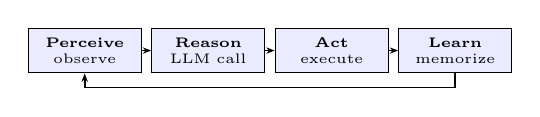
\begin{tikzpicture}[
    node distance=0.15cm,
    box/.style={rectangle, draw, fill=blue!8, text width=1.2cm, text centered, minimum height=0.45cm, font=\tiny},
    arrow/.style={-{Stealth[length=3pt]}, semithick},
]
    \node[box] (P) {\textbf{Perceive}\\observe};
    \node[box, right=0.12cm of P] (R) {\textbf{Reason}\\LLM call};
    \node[box, right=0.12cm of R] (A) {\textbf{Act}\\execute};
    \node[box, right=0.12cm of A] (L) {\textbf{Learn}\\memorize};
    \draw[arrow] (P) -- (R);
    \draw[arrow] (R) -- (A);
    \draw[arrow] (A) -- (L);
    \draw[arrow] (L.south) -- ++(0,-0.18) -| (P.south);
\end{tikzpicture}
\caption{The PARL decision trace loop.}
\label{fig:parl}
\end{figure}

\subsection{Trace Points and Logging}

Table~\ref{tab:trace} summarizes the data captured at each stage of the PARL loop.

\begin{table}[ht]
\centering
\caption{Traceability capture points.}
\label{tab:trace}
\scriptsize
\begin{tabular}{@{}lp{4.8cm}@{}}
\toprule
\textbf{Function} & \textbf{Data Captured} \\
\midrule
perceive()     & Agents seen, time, location, events \\
reason()       & LLM prompt, raw response, JSON action \\
execute()      & Action type, target, success/failure \\
add\_memory()   & Content, type, importance, agents \\
handle\_move()  & A* path, origin, destination, time \\
activity\_log   & All actions broadcast to frontend \\
\bottomrule
\end{tabular}
\end{table}

\subsection{Cognitive State Traceability}

Each agent maintains a full \textbf{CognitiveState} that acts as a persistent trace of the agent's mental state: \textbf{Identity Stable Set} (name, role, Big Five personality, backstory), \textbf{Action State} (status, description, emoji, duration), \textbf{Path State} (planned path, position, A* trace), \textbf{Conversation State} (partner, end time, cooldowns), and full serialization via \texttt{to\_dict()} / \texttt{from\_dict()} for replay and debugging.

\subsection{Memory Stream as Audit Trail}

The agent's local \textbf{memory stream} and global \textbf{MemoryStore} (FAISS-indexed) together form a complete audit trail. Every observation, action outcome, and reflection is timestamped with an importance score (1--10). The API endpoint \texttt{/api/agents/\{n\}/memories} exposes this trail for post-hoc analysis of decision chains.

\subsection{Anti-Repetition and Sanitization}

The PARL engine maintains per-agent action history (last 3 actions) and a sanitization pipeline that logs: hallucination corrections, invalid action fixes, target validation, and loop-breaking interventions via emoji-tagged console traces ([Move], [Conv], [Action], [Arrive]).

%===========================================================
\section{Simple Task Completion}
%===========================================================

\subsection{Task Lifecycle}

Each agent completes tasks autonomously through the simulation engine's processing pipeline:

\begin{enumerate}
    \item \textbf{Idle Detection:} When the current action completes, the agent enters reasoning.
    \item \textbf{LLM Decision:} PARL builds a context-rich prompt and calls the LLM, which returns a JSON decision with action, target, thought, and dialogue fields.
    \item \textbf{Execution:} Dispatched to the appropriate handler:
    \begin{itemize}
        \item \textbf{Move:} A* pathfinding, sets path and travel duration, teleports on completion.
        \item \textbf{Talk:} Validates target, initiates bidirectional conversation with timed duration.
        \item \textbf{Work:} Timed role-appropriate action.
        \item \textbf{Rest:} Short rest duration.
    \end{itemize}
    \item \textbf{Completion:} Agent stores a memory (``Finished \textit{task}'') and re-enters reasoning.
\end{enumerate}

\subsection{Verified Task Completions}

The following tasks were verified via API during live simulation runs (Table~\ref{tab:tasks}).

\begin{table}[ht]
\centering
\caption{Verified task completions from live simulation.}
\label{tab:tasks}
\scriptsize
\begin{tabular}{@{}llp{2.0cm}@{}}
\toprule
\textbf{Agent} & \textbf{Task} & \textbf{Outcome} \\
\midrule
Dr. Ananya Iyer & Move: Agri Lab  & Arrived; memorized \\
Rohan Kapoor    & Move: Comms     & Arrived; working \\
TARA            & Talk: Vikram    & Dialogue generated \\
Kabir Ahmed     & Talk: Vikram    & Conversation done \\
Dr. Priya Nair  & Move: Mess Hall & Arrived; reviewed \\
Dr. Arjun Reddy & Move: Med Bay   & Arrived (teleport) \\
Cdr. Vikram     & Work: logs      & Completed; stored \\
\bottomrule
\end{tabular}
\end{table}

\subsection{Conversation Trace Example}

\begin{lstlisting}[language={}]
[PARL] TARA decided: talk (Vikram)
[Conv] TARA -> Vikram (ends 06:42)
  "Good afternoon, Commander.
   All systems nominal."
[Conv] Ended. Memory stored.
\end{lstlisting}

%===========================================================
\section{Conclusion}
%===========================================================

The Chandrayaan-5 simulation demonstrates robust \textbf{tool integration} through 15+ REST/WebSocket endpoints and three interchangeable LLM providers with FAISS-powered semantic memory. \textbf{Agentic traceability} is achieved via PARL per-step logging, serializable cognitive state, memory audit trails, and structured console traces. \textbf{Task completion} is verified through autonomous decision-making, A* pathfinding, timed execution, and memory-backed recording --- validated with eight concurrent agents.

\begin{thebibliography}{9}\itemsep=0pt\parskip=0pt
\bibitem{park2023}
J.~S.~Park \textit{et al.}, ``Generative agents: Interactive simulacra of human behavior,'' \textit{Proc. UIST}, 2023.
\bibitem{russell2020}
S.~Russell and P.~Norvig, \textit{AI: A Modern Approach}, 4th~ed., Pearson, 2020.
\end{thebibliography}

\end{document}
